\let\negmedspace\undefined
\let\negthickspace\undefined
\documentclass[journal,12pt,onecolumn]{IEEEtran}
\usepackage{cite}
\usepackage{amsmath,amssymb,amsfonts,amsthm}
\usepackage{algorithmic}
\usepackage{graphicx}
\usepackage{textcomp}
\usepackage{xcolor}
\usepackage{txfonts}
\usepackage{listings}
\usepackage{enumitem}
\usepackage{mathtools}
\usepackage{gensymb}
\usepackage[breaklinks=true]{hyperref}
\usepackage{tkz-euclide} % loads  TikZ and tkz-base
\usepackage{listings}



\newtheorem{theorem}{Theorem}[section]
\newtheorem{problem}{Problem}
\newtheorem{proposition}{Proposition}[section]
\newtheorem{lemma}{Lemma}[section]
\newtheorem{corollary}[theorem]{Corollary}
\newtheorem{example}{Example}[section]
\newtheorem{definition}[problem]{Definition}
%\newtheorem{thm}{Theorem}[section] 
%\newtheorem{defn}[thm]{Definition}
%\newtheorem{algorithm}{Algorithm}[section]
%\newtheorem{cor}{Corollary}
\newcommand{\BEQA}{\begin{eqnarray}}
\newcommand{\EEQA}{\end{eqnarray}}
\newcommand{\define}{\stackrel{\triangle}{=}}
\theoremstyle{remark}
\newtheorem{rem}{Remark}
%\bibliographystyle{ieeetr}
\begin{document}
%
\providecommand{\pr}[1]{\ensuremath{\Pr\left(#1\right)}}
\providecommand{\prt}[2]{\ensuremath{p_{#1}^{\left(#2\right)} }}        % own macro for this question
\providecommand{\qfunc}[1]{\ensuremath{Q\left(#1\right)}}
\providecommand{\sbrak}[1]{\ensuremath{{}\left[#1\right]}}
\providecommand{\lsbrak}[1]{\ensuremath{{}\left[#1\right.}}
\providecommand{\rsbrak}[1]{\ensuremath{{}\left.#1\right]}}
\providecommand{\brak}[1]{\ensuremath{\left(#1\right)}}
\providecommand{\lbrak}[1]{\ensuremath{\left(#1\right.}}
\providecommand{\rbrak}[1]{\ensuremath{\left.#1\right)}}
\providecommand{\cbrak}[1]{\ensuremath{\left\{#1\right\}}}
\providecommand{\lcbrak}[1]{\ensuremath{\left\{#1\right.}}
\providecommand{\rcbrak}[1]{\ensuremath{\left.#1\right\}}}
\newcommand{\sgn}{\mathop{\mathrm{sgn}}}
\providecommand{\abs}[1]{\left\vert#1\right\vert}
\providecommand{\res}[1]{\Res\displaylimits_{#1}} 
\providecommand{\norm}[1]{\left\lVert#1\right\rVert}
%\providecommand{\norm}[1]{\lVert#1\rVert}
\providecommand{\mtx}[1]{\mathbf{#1}}
\providecommand{\mean}[1]{E\left[ #1 \right]}
\providecommand{\cond}[2]{#1\middle|#2}
\providecommand{\fourier}{\overset{\mathcal{F}}{ \rightleftharpoons}}
\newenvironment{amatrix}[1]{%
  \left(\begin{array}{@{}*{#1}{c}|c@{}}
}{%
  \end{array}\right)
}
%\providecommand{\hilbert}{\overset{\mathcal{H}}{ \rightleftharpoons}}
%\providecommand{\system}{\overset{\mathcal{H}}{ \longleftrightarrow}}
	%\newcommand{\solution}[2]{\textbf{Solution:}{#1}}
\newcommand{\solution}{\noindent \textbf{Solution: }}
\newcommand{\cosec}{\,\text{cosec}\,}
\providecommand{\dec}[2]{\ensuremath{\overset{#1}{\underset{#2}{\gtrless}}}}
\newcommand{\myvec}[1]{\ensuremath{\begin{pmatrix}#1\end{pmatrix}}}
\newcommand{\mydet}[1]{\ensuremath{\begin{vmatrix}#1\end{vmatrix}}}
\newcommand{\myaugvec}[2]{\ensuremath{\begin{amatrix}{#1}#2\end{amatrix}}}
\providecommand{\rank}{\text{rank}}
\providecommand{\pr}[1]{\ensuremath{\Pr\left(#1\right)}}
\providecommand{\qfunc}[1]{\ensuremath{Q\left(#1\right)}}
	\newcommand*{\permcomb}[4][0mu]{{{}^{#3}\mkern#1#2_{#4}}}
\newcommand*{\perm}[1][-3mu]{\permcomb[#1]{P}}
\newcommand*{\comb}[1][-1mu]{\permcomb[#1]{C}}
\providecommand{\qfunc}[1]{\ensuremath{Q\left(#1\right)}}
\providecommand{\gauss}[2]{\mathcal{N}\ensuremath{\left(#1,#2\right)}}
\providecommand{\diff}[2]{\ensuremath{\frac{d{#1}}{d{#2}}}}
\providecommand{\myceil}[1]{\left \lceil #1 \right \rceil }
\newcommand\figref{Fig.~\ref}
\newcommand\tabref{Table~\ref}
\newcommand{\sinc}{\,\text{sinc}\,}
\newcommand{\rect}{\,\text{rect}\,}
%%
%	%\newcommand{\solution}[2]{\textbf{Solution:}{#1}}
%\newcommand{\solution}{\noindent \textbf{Solution: }}
%\newcommand{\cosec}{\,\text{cosec}\,}
%\numberwithin{equation}{section}
%\numberwithin{equation}{subsection}
%\numberwithin{problem}{section}
%\numberwithin{definition}{section}
%\makeatletter
%\@addtoreset{figure}{problem}
%\makeatother

%\let\StandardTheFigure\thefigure
\let\vec\mathbf


\bibliographystyle{IEEEtran}
\title{ GATE CH-23 44}
\author{EE23BTECH11011- Batchu Ishitha$^{*}$% <-this % stops a space
}
\maketitle




\bigskip

\renewcommand{\thefigure}{\theenumi}
\renewcommand{\thetable}{\theenumi}
%\renewcommand{\theequation}{\theenumi}

Q: A cascade control strategy is shown in the figure below. The transfer function between the output $(y)$ and the secondary disturbance $(d_2)$ is defined as  \\


$$G_{d2}(s)= \frac{y(s)}{d_2(s)}$$. 


Which one of the following is the CORRECT expression for the transfer function $G_{d2}(s)$? \\

\begin{figure}[h]
    \centering
    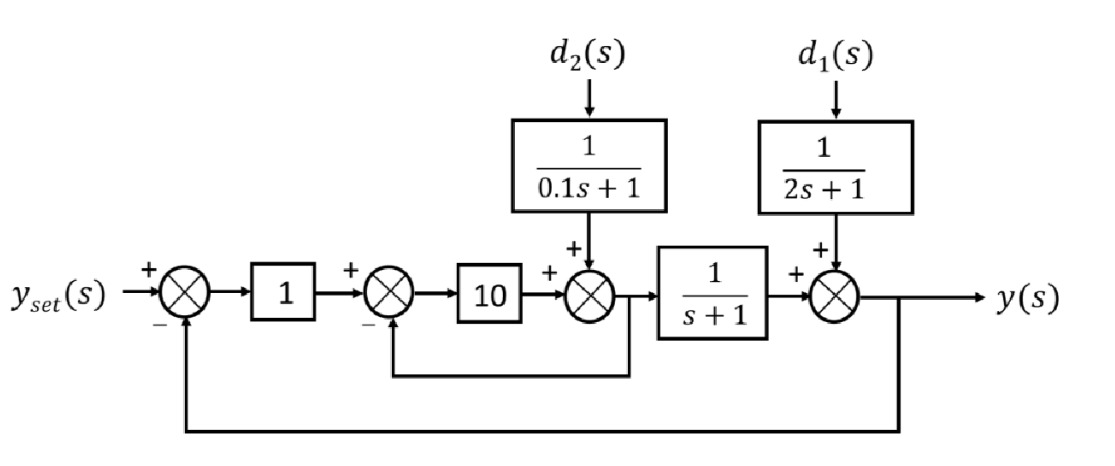
\includegraphics[scale=0.25]{../gate23.ch.44/figs/g44fig1.jpeg}
    \caption{ }
    \label{}
\end{figure}

\begin{enumerate}[label=\Alph*.]
\item $\frac{1}{(11s+21)(0.1s+1)}$ 
\item $\frac{1}{(s+1)(0.1s+1)}$
\item $\frac{(s+1)}{(s+2)(0.1s+1)}$
\item $\frac{(s+1)}{(s+1)(0.1s+1)}$
\end{enumerate}

\solution 

\begin{table}[!ht]
    \centering
              \begin{tabular}{|c|c|c|} 
      \hline
\textbf{Variable}& \textbf{Description}& \textbf{Value}\\\hline
         $y(s)$& output &none\\\hline
         $d_2(s)$& Secondary disturbance &none\\\hline
         $G_{d2}(s)$&Transfer function between $y(s)$ and $d_2(s)$&$\frac{y(s)}{d_2(s)}$\\\hline
              \end{tabular}

    \caption{Input Parameters}
    \label{tab: ishithagatech44.t1}
\end{table}

\begin{equation}
\sbrak{\brak{y_{sp}-y}(1) -a}10+ d_2(s)\frac{1}{0.1s+1} =a \\ \label{eq:ishitha.g23.ch44.1.eq}
\end{equation}

\begin{equation}
a\brak{\frac{1}{s+1}} + d_1(s)\frac{1}{(2s+1)} =y \\  \label{eq:ishitha.g23.ch44.2.eq}
\end{equation}

From~\eqref{eq:ishitha.g23.ch44.1.eq}
\begin{align}
\brak{y_{sp}-y}10 -10a + d_2(s)\frac{1}{0.1s+1}&=a \\
\brak{y_{sp}-y}10 + \frac{d_2(s)}{0.1s+1} =11a 
\end{align}

\begin{equation}
\brak{y_{sp}-y}\frac{10}{11} + \frac{d_2(s)}{11\brak{0.1s+1}} = a \\ \label{eq:ishitha.g23.ch44.3.eq}
\end{equation}

Substituting ~\eqref{eq:ishitha.g23.ch44.3.eq} in ~\eqref{eq:ishitha.g23.ch44.2.eq}
\begin{align}
\sbrak{\brak{y_{sp}-y}\frac{10}{11} + \frac{d_2(s)}{11\brak{0.1s+1}}  }\frac{1}{\brak{s+1}} + d_1(s)\frac{1}{(2s+1)} &= y \\
\brak{y_{sp}-y}\frac{10}{11}\frac{1}{\brak{s+1}} + \frac{d_2(s)}{11\brak{0.1s+1}\brak{s+1}} +  d_1(s)\frac{1}{(2s+1)} &= y 
\end{align} 

\begin{align}
\brak{0-y}\frac{10}{11}\frac{1}{\brak{s+1}} + \frac{d_2(s)}{11\brak{0.1s+1}\brak{s+1}} &= y \\
\frac{d_2(s)}{11\brak{0.1s+1}\brak{s+1}} &= y + \frac{10}{11}y\frac{1}{\brak{s+1}} \\
\frac{d_2(s)}{11\brak{0.1s+1}\brak{s+1}} &= y(s)\brak{1 + \frac{10}{11}\frac{1}{\brak{s+1}}} \\
\frac{d_2(s)}{11\brak{0.1s+1}\brak{s+1}} &= y(s)\brak{\frac{11\brak{s+1}+10}{11\brak{s+1}}} \\
\frac{d_2{s}}{\brak{0.1s+1}} &= y(s)\sbrak{11s+ 11 +10} \\
\frac{d_2{s}}{\brak{0.1s+1}} &= y(s)\sbrak{11s+21} \\
\frac{y(s)}{d_2{s}} &= \frac{1}{\brak{0.1s+1}\brak{11s+21}} \\
\implies G_{d2}(s) &= \frac{1}{\brak{0.1s+1}\brak{11s+21}}
\end{align}
\end{document}
